\section*{Sobre a carta da Comissão de Recepção}
\autoria{anônimo}
\avisoTextoForms

As Gincanas da Semana de Recepção do IME é um evento que ocorre todo início de ano, e sempre conta com a participação de veteranos e calouros em uma série de atividades, palestras e jogos projetadas para enturmar a calourada e fazê-la conhecer os espaços do IME e da própria USP. Organizada pela Comissão de Recepção, um tema é sempre decidido no ano anterior para o ano consequente. Em 2022, o tema escolhido foi Shrek; em 2023, foi Scooby- doo; e assim por diante. Para acomodar as temáticas escolhidas, são feitas identidades e dicas visuais usando tanto figuras em si de cada tema, como também cores que representam o tema. Além disso, as atividades programadas e todo aparato adjacente das atividades - premiação, nome da atividade, formato, etc - também acompanham a temática escolhida.

Neste ano de 2024, a Comissão acabou por optar na escolha do tema de Kung Fu Panda, aproveitando o esperado lançamento do quarto filme da franquia nos cinemas. Por se tratar de uma franquia que, de muitos modos, possibilita uma aproximação com a ideia de “Kung Fu na visão do Ocidente”, e existem nela elementos que inevitavelmente podem remeter ao senso-comum sobre o que é Kung Fu, o que é China, e principalmente no reforço de uma ideia visual de “Oriente-extremo” como um todo quando se toma uma visão descuidada na sua interpretação. Para isso, basta observar como a filosofia de Kung Fu é retratada em peças de mídia chinesa e em Kung Fu Panda.

A partir de contos, poemas e histórias dentro dos vários universos literários chineses, a ideia de Kung Fu é retratada de maneira a não glorificar violência e tecnicalidades. Kung Fu, na literatura chinesa, é interpretado como um estado de ser que foca na iluminação intelectual. A própria palavra Kung Fu no seu sentido literal não sugere estritamente luta, mas sim “fundamentos” - para qualquer coisa -. A sua tradução ao pé da letra pode ser entendida como “habilidade” ou “saber de algo”, ao ponto do termo ser usado como expressão para alguém habilidoso: “Uau! Você realmente dedicou kung fu nos estudos!”.

Em contraste, Kung Fu Panda parece inevitavelmente seguir o tropo hollywoodiana do Escolhido: um herói inserido em um mundo estranho, conhece um mentor, descobre aliados, e combate o mal. Aqui, Kung Fu é visto como um conjunto de técnicas que necessariamente existem para aperfeiçoar a fisicalidade da luta e somente: os Cinco Furiosos são reverenciados pela sua agilidade, força e ferocidade, e são de fato tratados como estrelas de filme; e o Po é visto como um instrumento para derrotar o vilão. Assim, Kung Fu Panda não é um filme sobre a China.

É nesse contexto que a Comissão de Recepção 2024 escreve no Relatório da Semana de Recepção aos Calouros enviado à pró-reitoria que “[…​] Logo após tais premiações, a equipe com a maior pontuação obtida ao longo da gincana foi premiada com macarrão instantâneo e hashi, muito comuns na culinária chinesa, fazendo assim referência a temática da semana de recepção Kung-fu Panda […​]”.

Por um, o relatório dá a entender que existe uma unicidade na culinária chinesa, que não condiz com a realidade. Hoje, são oficialmente reconhecidos pelo Estado da República Popular da China 56 do que ficou traduzido como “etnias” dentro do seu território continental, e a sua diversidade se mostra em todos os aspectos possíveis: desde cultural, religioso, fenotípico e, claro, alimentar. Enquanto que os Han fazem o consumo normal de carne suína, por exemplo, os Hui - que representam, a depender da província, até 90\% da população local - não fazem por ser uma etnia tradicionalmente islâmica-sunita. Nesse sentido, é um erro assumir que existe somente uma China, pois de fato existem várias “Chinas”, sendo esta uma análise necessária a se ter consciência.

Em segundo plano, o aspecto mais gritante ao afirmar que macarrões instantâneos são “muito comuns na culinária chinesa” é o reforço dos estereótipos construídos ao longo da história sobre aquilo que se entende por China no Brasil, agravado pela ideia do uso de Hashi. Claro que macarrões são consumidos na China, e constitui um dos pilares alimentares das várias culturas que coexistem e intersectam, e de fato utensílios parecidos com Hashi são usados. Porém, a maneira como macarrões instantâneos existem no Brasil não é um reflexo fiel do alimento consumido na China, tampouco o uso do termo Hashi demonstra uma preocupação em entender a origem do termo no contexto histórico brasileiro quanto à vinda e presença desses imigrantes. Foi ignorada, nesse aspecto, a existência de erros fundamentais de coerência histórica e linguística. O macarrão instantâneo encontrado nos mercados de hoje é uma invenção japonesa - fato verificável com uma rápida busca de 4 segundos -. O termo “Hashi”, também, é a transliteração japonesa para o utensílio. Claro que, mecanicamente, Hashi e Kuaizi são muito parecidos. Mas conceitualmente e, de certa forma, culturalmente não são, uma vez que a linguagem não é neutra. O fato do utensílio ser oficializado no Brasil como Hashi e não Kuaizi ou Jeotgarak vem de uma disputa histórica pelo domínio da narrativa sobre quem define o que é o “oriental”. Não à toa que na Zona Central de São Paulo existe a Praça da Liberdade África-Japão que, além de colocar África como em igual status de país justaposta ao Japão, faz parecer que existe uma predominância japonesa na região - o que não é verdade -.

Tudo isso e outros problemas são, em essência, frutos de uma análise inefetiva da franquia que foi usada como tema para a Semana. Assim, retoma-se a discussão sobre Kung Fu Panda não ser um filme sobre a China: a franquia nunca se propôs a ser. A construção de mundo e narrativa em Kung Fu Panda é, nas palavras do co-diretor do primeiro filme John Stevenson, “[…​] Vamos fazê-lo um filme de artes marciais de verdade, um que tenha um personagem cômico […​]”. Kung Fu Panda, em essência, é uma carta de apreciação que os produtores dedicaram aos filmes de Kung Fu - filmes estes que os próprios produtores cresceram assistindo -; e nisso, Kung Fu Panda se mostrou detalhista e respeitável quando, ao longo da franquia, são usadas de maneira respeitosa referências cinematográficas que trazem memórias do que a indústria cinematográfica de Hong Kong uma vez foi. O design de Po é, para além da quebra da ideia de que somente o mais fisicamente apto pode praticar lutas, é também uma referência ao cinema de Sammo Huang; muitas cenas fazem uma releitura de Kung-Fusão de Stephen Chow; o uso livre de objetos como parte da luta é uma referência ao humor de Jackie Chan.

Sobre isso, a Comissão cometeu um erro de leitura ao entender Kung Fu Panda como “China”, agravado pelo uso de elementos que flertam com um processo histórico de racismo. A própria fonte utilizada nas artes e postagens evocam um senso de “orientalidade” através de uma espécie de reinterpretação de traços da escrita chinesa adaptados para escrever o alfabeto latino. Dentro do design gráfico, esse tipo de fonte é chamado de “fontes wonton” ou “fontes chop-suey”, um sub-gênero da família de “fontes étnicas”, desenhadas para criar uma identidade visual que seja associada a grupos étnicos específicos: como a fonte que evoca uma ideia de “África” usada nos cartazes para O Rei Leão - O Musical. É a equivalência escrita de sotaques estereotipados, ainda mais considerando a origem indubitavelmente reducionista de fontes chop-suey e da maneira como a associação da identidade chinesa a essas fontes serviram de aparatos para terceirizar e desumanizar estes imigrantes ao longo dos séculos XVIII, XIX e XX. Nisso, vale a pena notar que Kung Fu Panda não faz o uso desse tipo de fonte em seus cartazes. 

\begin{figure}[H]
    \centering
    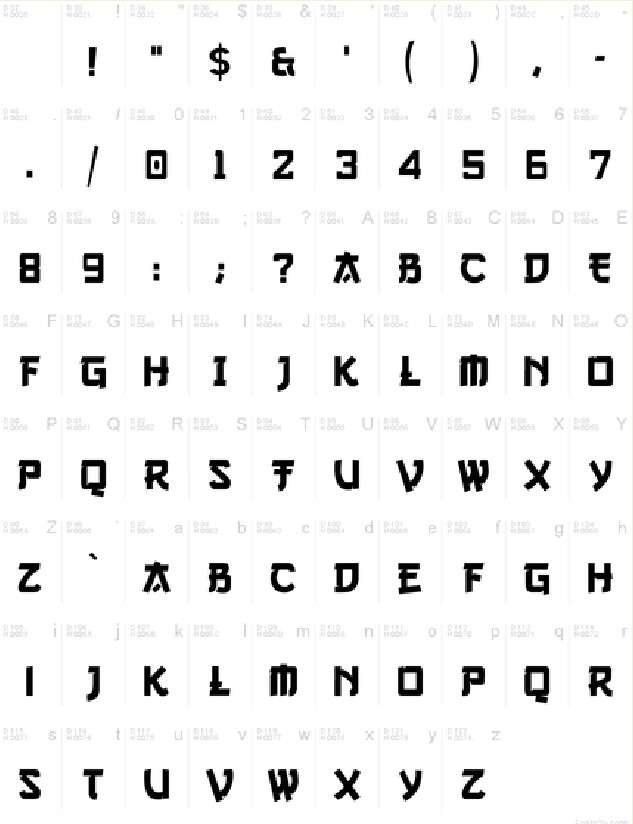
\includegraphics[width=0.7\linewidth]{textos/img/exemplo_chop_suey_gang_of_three.jpg}
    \legendaFigura{1}{\textit{"Gang of Three", exemplo de uma fonte chop-suey.}}
\end{figure}

Assim, percebe-se que, para além de ter um olhar mais sensível de entender as nuances históricas e entender que linguagem não é só o texto pleno que foi escrito, mas também a sua apresentação estética, é importante, também, fazer uma interpretação mais acurada das obras e franquias que virão a ser temas quando envolve algum elemento que não seja familiar aos membros da Comissão, seja este uma cultura nova, uma identidade nova, um visual novo; de ter a paciência de perguntar e entender: o que essa obra realmente quer dizer? 